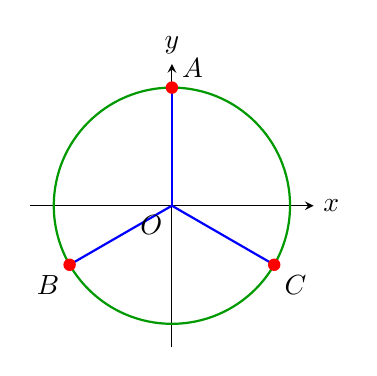
\begin{tikzpicture}[>=stealth, scale=1.5]
    \draw[->] (-1.2,0) -- (1.2,0)  node[right] {$x$};
    \draw[->] (0,-1.2) -- (0,1.2)  node[above] {$y$};
    \draw[green!60!black, thick] (0,0) circle (1);
    \coordinate (A) at (90:1);
    \coordinate (B) at (210:1);
    \coordinate (C) at (330:1);
    \draw[blue, thick] (0,0) -- (A) node[above right, black] {$A$};
    \draw[blue, thick] (0,0) -- (B) node[below left, black] {$B$};
    \draw[blue, thick] (0,0) -- (C) node[below right, black] {$C$};
    \fill[red] (A) circle (1.5pt);
    \fill[red] (B) circle (1.5pt);
    \fill[red] (C) circle (1.5pt);
    \node[below left] at (0,0) {$O$};
\end{tikzpicture}